%================================================================================
%       Safety Critical Systems Club - Data Safety Initiative Working Group
%================================================================================
%                       DDDD    SSSS  IIIII  W   W   GGGG
%                       D   D  S        I    W   W  G   
%                       D   D   SSS     I    W W W  G  GG
%                       D   D      S    I    WW WW  G   G
%                       DDDD   SSSS   IIIII  W   W   GGG
%================================================================================
%               Data Safety Guidance Document - LaTeX Source File
%================================================================================
%
% Description:
%   Appendix addressing data migration
%================================================================================
\section{Data Migrating, Porting, Importing and Exporting (Informative)}\index{Data Migration}\label{bkm:migration}
%
%\dsiwgSectionQuote{The whole story of migration and what that has done in interconnecting the planet is obviously something I've written about a lot}{Salman Rushdie}
%\dsiwgSectionQuote{Migration is an expression of the human aspiration for dignity, safety and a better future. It is part of the social fabric, part of our very make-up as a human family}{Ban Ki-moon}
%\dsiwgSectionQuote{When it's well managed, migration works in the national interest, for our communities, economy and country.}{Priti Patel}
%\dsiwgSectionQuote{I think migration is a right, but it should be an option, not an obligation}{Nayib Bukele}
\dsiwgSectionQuote{I don't think you'll ever have a perfect world because we humans are prone to error, and so we're always in search of an upgrade}{Henry Rollins}

Migrating, Porting and Import or Export of data between systems is a large and complex topic.
This appendix highlights some of the issues that arise, links to the data safety properties and suggests some mitigations.

\subsection{Introduction and rationale}\label{bkm:migrationintro}
All of these activities involve moving data around, with the expectation that the data will be re-used or re-purposed to some extent after the move. Why is this a problem? Because data can be lost, transformed or misinterpreted due to the migration. If some of this data is safety-related then there is the possibility of creating a data \gls{hazard}. The worst cases are the silent ones: where data is not migrated or modified or changed into something else on migration, and no notification or warning is provided.
In general porting of data, import and export actions can be considered subsets of full data migration activities. 
The following are typical stages of a data migration exercise:
\begin{enumerate}[label=\color{dsiwgAccentColour}\roman*)]
\item Discovery: Identifying what data has to be migrated:
the history, locations, store types, formats and the software currently used to manipulate it.
\item Analysis and Preparation:
Filtering and sorting the data, identifying and cleansing the data, fixing any issues, creating missing data that can’t be moved,
and transforming the data to make it suitable for use in the new system.
\item Trials:
Selected sets or portions of the data are migrated and the results assessed within the new system or context.
This may be extended to include more data through incremental, phased stages.
\item Dry Run:
A full migration is performed to a duplicate system or to the new system in a way that it can be backed out
(ie. the new system can be reverted to its original state), and use of the current system can be continued if necessary.
\item Parallel Running:
Both old and new systems continue running, processing the same data where possible.
This is desirable as it allows quick reversion to the old system in case of failure.
It also allows (sampling) comparison between the old and new systems outputs.
\item Monitoring and Checking:
Operation of the new system is closely monitored and outputs assessed to establish if these would be similar to those produced
by the old system.
\item Move to New:
This is where the old system is switched off and mothballed, and may be subsequently decommissioned and removed.
\end{enumerate}

It is noted that migration is generally between systems
(e.g. a legacy system and a new one) but can be between different instances or environments within the same system,
involving different software, stores or \glspl{database}.

Many moves of data are now to Cloud storage, and the implementation may be largely hidden,
with only software API interfaces available\footnote{It is noted that within a cloud environment mini automated migrations of data are happening all the time as new servers and storage are provisioned by the service provider, software is upgraded, etc. There should be some sort of assurance provided in this case to ensure the data is preserved as required.}.
In this case the options for comparisons may be more limited.
%
\subsection{Migration Cases}
%
There are at least three cases of migration (these simple diagrams are intended to show the end state of the migration, it is acknowledged that there are intermediate stages, as mentioned in \dsiwgRef{Section}{bkm:migrationintro}):
\begin{enumerate}
\item Migration of data from a single old system to a single new system.
This is very common and is the usual upgrade path.
The new system, or indeed both systems, may be in the Cloud.

\begin{figure}[htbp]
  \centering
  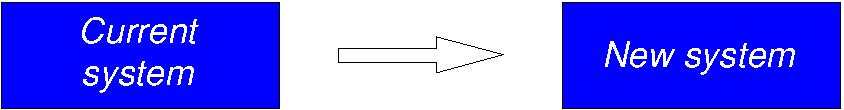
\includegraphics[width=\textwidth/2]{images/migration1.pdf}
  \caption{Simple Migration Path\index{Data Migration!Simple}}
  \label{fig:migration1}
\end{figure}

\item Migration of data from multiple disparate systems to one new system.
This is less common but can be seen in major technology upgrades where it is seen as beneficial to bring together multiple
legacy systems into one new system.

\begin{figure}[htbp]
  \centering
  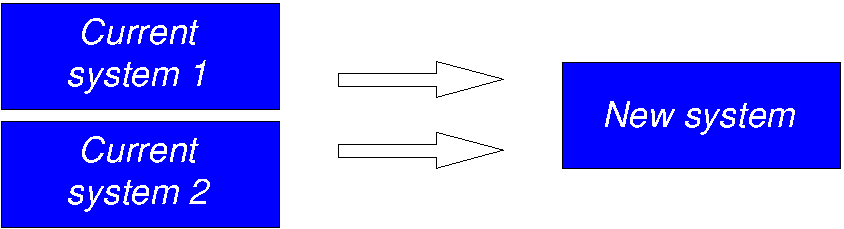
\includegraphics[width=\textwidth/2]{images/migration2.pdf}
  \caption{Many-to-one Migration Path\index{Data Migration!Many to one}}
  \label{fig:migration2}
\end{figure}

\item Migrating data back to an old system in case of failures or to investigate data issues with the new system

\begin{figure}[htbp]
  \centering
  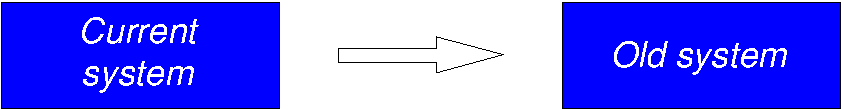
\includegraphics[width=\textwidth/2]{images/migration3.pdf}
  \caption{Reversion Migration Path\index{Data Migration!Reversion}}
  \label{fig:migration3}
\end{figure}

\end{enumerate}
%
\subsection{Safety Issues due to Migration}
%
The following table summarises some of the safety issues due to migration, maps these to the data safety properties and gives possible mitigations.

\begin{longtable}{|C{\dsiwgColumnWidth{0.10}}|C{\dsiwgColumnWidth{0.24}}|C{\dsiwgColumnWidth{0.20}}|C{\dsiwgColumnWidth{0.20}}|C{\dsiwgColumnWidth{0.20}}|}
  \caption{Safety Issues due to Migration}
  \label{tab:migration}
  \\\hline
  \TableHeadColourCX{No.} & \TableHeadColourCX{Migration Case} & \TableHeadColourCX{What are safety issues in each case?} & \TableHeadColourCX{Mapping to properties/loss of properties} & \TableHeadColourCX{Possible Mitigations (Table \ref{tab:MethodsDataMigration})}\\\hline
  \endfirsthead
  \caption[]{Safety Issues due to Migration (continued)}
  \\\hline
  \TableHeadColourCX{No.} & \TableHeadColourCX{Migration Case} & \TableHeadColourCX{What are safety issues in each case?} & \TableHeadColourCX{Mapping to properties/loss of properties} & \TableHeadColourCX{Possible Mitigations (Table \ref{tab:MethodsDataMigration})}\\\hline
  \endhead
  \multicolumn{5}{r}{\sl Continued on next page}
  \endfoot
  \endlastfoot

1.&
Data format may not map exactly: due to different \gls{database} formats, word lengths, endian issues, etc.&
Data can be lost or discarded, or substituted for defaults. Data may be migrated / imported / exported incorrectly.&
\Gls{integrity}, \gls{completeness}, Format&
DM.02, DM.07, DM.08, DM.09, DM.10\\\hline
%
2.&
Data may not translate exactly: no equivalent data type / record / field type in new system, etc&
Data can be lost or discarded, or substituted for defaults. Data may be migrated / imported / exported incorrectly.&
\Gls{integrity}, \gls{completeness}&
DM.02, DM.04, DM.07, DM.08, DM.09, DM.10\\\hline
%
3.&
Data may not be valid: less numeric range available in new system, etc. Subtype of (2).&
Data can be lost or discarded, or substituted for defaults. Data may be migrated / imported / exported incorrectly.&
\Gls{integrity}, \gls{completeness}&
DM.02, DM.04, DM.07, DM.08, DM.09, DM.10\\\hline
%
4.&
\Gls{metadata} (data about the data) may be lost, including \gls{data dictionary} aspects, derivation, history, signoffs, authorisations,
logs, etc.&
Data may be migrated / imported / exported losing \gls{information}.&
Traceability, History&
DM.04, DM.09\\\hline
%
5.&
Data may have a different meaning or interpretation in the new system context.
E.g. if a fluid value is ‘gallons’ and this is migrated from a UK to a US-developed system without applying an adjustment factor.&
Meaning of data can be altered even if migration apparently successful.&
\Gls{consistency}, \gls{fidelity}&
DM.01, DM.04, DM.11\\\hline
%
6.
&
Data may be correctly rejected (detection of error on import/export)&
Data is lost. Not necessarily a problem if notified and fixed.&
\Gls{completeness}&
DM.07, DM.08, DM.09, DM.10\\\hline
%
7.
&
Data may be wrongly filtered or rejected as incompatible&
Correct data is rejected. If data can’t be imported what should happen? a. Rejected and migration halted,
b. Rejected and notified, c. Rejected silently, d. Substituted?&
\Gls{integrity}, \gls{completeness}&
DM.02, DM.03, DM.07, DM.08, DM.09, DM.10\\\hline
%
8.&
Two or more \glspl{item data} may map to the same item in the new system – one may overwrite the other with the last one ‘winning’.&
This is a case of aliasing (See 6.2.2 ref). Data can be lost or discarded. Data may be migrated / imported / exported incorrectly.&
\Gls{integrity}, \gls{completeness}&
DM.02, DM.03, DM.07, DM.08, DM.09, DM.10\\\hline
%
9.&
There may be situations where the data store has to be ‘live’ and the migration / import / export process takes some time.
In this case some data may be out of date and become inconsistent (stale), and \gls{integrity} of the whole data set is lost.&
Data may be migrated / imported / exported incorrectly.&
\Gls{consistency}, \gls{integrity}, Timeliness&
DM.07, DM.08\\\hline
%
10.&
If a migration is unsuccessful, data changes may have to be undone and stores reverted to original state.
This may not always be possible or completely done.&
Original data set may be corrupted.&
\Gls{consistency}, \Gls{integrity}&
DM.06, DM.07, DM.08\\\hline
%
11.&
The data ‘cleansing’ activity conducted before or during migration may introduce faults.&
The cleansing activity may miss some data faults or may be over-zealous, deleting good values.&
\Gls{integrity}, \gls{completeness}&
DM.07, DM.09, DM.13\\\hline
\end{longtable}
